%------------------------------------------------
% main.tex - MA1500 2015-16
%------------------------------------------------
\documentclass{camel}

% options (these don't work!)
% \cymraegtrue
% \screentrue
% \booklettrue
% \blankstrue
% \answerstrue

% module information
\academicyear{2015-16}
\modulecode{MA0000}
\moduletitle{Cardiff Maths e-Learning}

\booknumber{1}
\booktitle{User Guide}
\bookauthor{Dafydd Evans}
\bookversion{v0.1}

% figures
\usepackage{graphicx}
\graphicspath{{./figures/}}
\DeclareGraphicsExtensions{.pdf,.jpeg,.png,.gif}
\usepackage{caption}
\usepackage{subcaption}
\captionsetup[subfigure]{labelformat=empty}
\captionsetup[figure]{skip=2ex}

% naughty
\def\it{\item}
\def\bit{\begin{itemize}}
\def\eit{\end{itemize}} 
\def\ben{\begin{enumerate}}
\def\een{\end{enumerate}}

% macros
\newcommand{\Z}{\mathbb{Z}}
\newcommand{\N}{\mathbb{N}}
\newcommand{\R}{\mathbb{R}}
\newcommand{\C}{\mathbb{C}}


%------------------------------------------------
\begin{document}
\makefrontmatter

%------------------------------------------------
\chapter{Introduction}\label{ch:intro}
Welcome to the Cardiff Maths eLearning project.

BLAH

%------------------------------------------------
\chapter{Figures}\label{ch:figures}
Here is a nice picture of our sponsor.

\begin{figure}[ht]
\centering
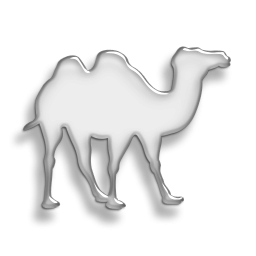
\includegraphics[scale=0.5]{camel_logo_reversed.png}
\caption{The Camel Project logo.}
\label{fig:camel-logo}
\end{figure}

No more figures.

%------------------------------------------------
\chapter{Lists}\label{ch:lists}

Initial text.
\begin{itemize}
\item First item of itemize list
\begin{enumerate}
\item First item of nested enumerate list.
\item Second item of nested enumerate list.
\end{enumerate}
\item Second item of itemize list
\end{itemize}
Final text.

%------------------------------------------------
\chapter{Labels, References and Citations}

\begin{itemize}
\item Here we include a label: \label{it:first-item}.
\item Here we include a reference to the introduction: Chapter~\ref{ch:intro}.
\item Here we include a citation: \cite{evans02}.
\end{itemize}

%------------------------------------------------
\chapter{Assessments}\label{ch:assessments}

\begin{assessment}\label{ass:demo}
This is the introduction to the assessment.
\begin{questions} 
\question This is the first question.\label{qu:first-question}
\begin{answer} 
This is an answer to the first question.
\end{answer} 
\question This is the second question.\label{qu:second-question}
\begin{answer} 
This is an answer to the second question.
\end{answer} 
\question This is the third question.\label{qu:third-question}
\begin{parts}
\part This is the first part of the third question
\begin{answer} 
This is an answer to the first part of the third question.
\end{answer} 
\part This is the second part of the third question
\begin{answer} 
This is an answer to the second part of the third question.
\end{answer} 
\end{parts}
\end{questions} 
\end{assessment}

%------------------------------------------------
\chapter{Theorems}\label{ch:theorems}
\begin{theorem}
\[
a^2 + b^2 = c^2
\]
\end{theorem}

\begin{exercise}
Can you fix it?
\end{exercise}

%------------------------------------------------
\chapter{MathJax}\label{ch:mathjax}
Let $\alpha$ and $\beta$ be ...
\[
\int_0^1 2x\,dx = 1. 
\]
Here is an equation with a label:
\begin{equation}\label{eq:einstein}
E = mc^2
\end{equation}

%------------------------------------------------
\end{document}
%------------------------------------------------

